% !TeX program = xelatex 
\documentclass{hitreport}
\usepackage{url}
\usepackage{algorithm,float}  
\usepackage{algpseudocode}  
\usepackage{amsmath}
\usepackage{cite}
\usepackage{threeparttable}
\usepackage{subfig}
\usepackage{listings} %插入代码
\usepackage{xcolor} %代码高亮
\usepackage{tikz}
\usetikzlibrary{shapes,arrows}
\usepackage{hyperref}
\usepackage{wasysym}
\usepackage{pgfplots}



\lstset{numbers=left, %设置行号位置
	numberstyle=\tiny, %设置行号大小
	keywordstyle=\color{blue}, %设置关键字颜色
	commentstyle=\color[cmyk]{1,0,1,0}, %设置注释颜色
	frame=single, %设置边框格式
	escapeinside=``, %逃逸字符(1左面的键),用于显示中文
	breaklines, %自动折行
	extendedchars=false, %解决代码跨页时,章节标题,页眉等汉字不显示的问题
	xleftmargin=2em,xrightmargin=2em, aboveskip=1em, %设置边距
	tabsize=4, %设置tab空格数
	showspaces=false %不显示空格
}

\tikzstyle{startstop} = [rectangle,rounded corners, minimum width=3cm,minimum height=1cm,text centered, draw=black,fill=red!30]
\tikzstyle{io} = [trapezium, trapezium left angle = 70,trapezium right angle=110,minimum width=3cm,minimum height=1cm,text centered,draw=black,fill=blue!30]
\tikzstyle{process} = [rectangle,minimum width=3cm,minimum height=1cm,text centered,text width =4cm,draw=black,fill=orange!30]
\tikzstyle{decision} = [diamond,minimum width=3cm,minimum height=1cm,text centered,draw=black,fill=green!30]
\tikzstyle{arrow} = [thick,->,>=stealth]


\renewcommand{\algorithmicrequire}{\textbf{Input:}}  % Use Input in the format of Algorithm  
\renewcommand{\algorithmicensure}{\textbf{Output:}} % Use Output in the format of Algorithm  

\makeatletter
\newenvironment{breakablealgorithm}
  {% \begin{breakablealgorithm}
   \begin{center}
     \refstepcounter{algorithm}% New algorithm
     \hrule height.8pt depth0pt \kern2pt% \@fs@pre for \@fs@ruled
     \renewcommand{\caption}[2][\relax]{% Make a new \caption
       {\raggedright\textbf{\ALG@name~\thealgorithm} ##2\par}%
       \ifx\relax##1\relax % #1 is \relax
         \addcontentsline{loa}{algorithm}{\protect\numberline{\thealgorithm}##2}%
       \else % #1 is not \relax
         \addcontentsline{loa}{algorithm}{\protect\numberline{\thealgorithm}##1}%
       \fi
       \kern2pt\hrule\kern2pt
     }
  }{% \end{breakablealgorithm}
     \kern2pt\hrule\relax% \@fs@post for \@fs@ruled
   \end{center}
  }
\makeatother

% =============================================
% Part 0 Edit the info
% =============================================

\major{计算机科学与技术}
\name{孙骁}
\title{视听觉信号处理\\实验报告}
\stuid{1180300811} % 学号
\college{计算学部}
\date{2020年11月18日}
\lab{} %实验地点
\course{视听觉信号处理}
\instructor{姚鸿勋}
% \grades{}
\expname{实验三} %实验名称
% \exptype{} % 实验类型
% \partner{} % 同组学生名字
\term{2020秋季学期}

\begin{document}

\maketitle

\tableofcontents
\newpage
% =============================================
% Part 1 Header
% =============================================



% =============================================
% Part 2 Main document
% =============================================

\section{实验目标和内容}

\subsection{实验目标}
\begin{enumerate}
\item 综合运用图像处理的知识解决实际问题,以及可能出现的多种多样的
情况。
\end{enumerate}

\subsection{实验内容}
\begin{enumerate}
\item 对给定的静止状态下的一辆汽车图像进行车牌定位与检测,框出车牌保存结果图像,描述清楚整个算法流程;
\item (选做)在现实情况下,我们可能存在多种多样的情况。高速移动下的车牌;晚上夜景下的车牌;车牌的某些字符部分遮挡;图片中含有多张车牌;车牌倾斜情况。可以从中挑出一个感兴趣的去尝试进行定位(不仅限于上述情况)。
\end{enumerate}

\section{实验环境}

\begin{enumerate}
\item Anaconda 4.8.4
\item Python 3.7.4
\item PyCharm 2019.1 (Professional Edition)
\item Windows 10 2004
\end{enumerate}

\section{实验原理}

\subsection{腐蚀}\label{sec:corrosion}

腐蚀是经典的形态学操作。假设\textit{A}和\textit{B}是$Z^2$中的两个集合,\textit{B}对\textit{A}的腐蚀定义为
\begin{align}\label{equ:AominusB}
A\ominus B = \left\{z | \left(B\right)_z\subseteq A\right\},
\end{align}
式中,\textit{A}是前景像素的一个集合,\textit{B}是一个结构元,\textit{z}项是前景像素值。公式(\ref{equ:AominusB})指出\textit{B}对\textit{A}的腐蚀是所有点\textit{z}的集合,条件是平移后的\textit{B}包含于\textit{A}。

腐蚀可以用于消除物体边界点,使目标缩小,可以消除小于结构元素的噪声点。

\subsection{膨胀}\label{sec:swell}

膨胀是腐蚀的对偶运算。假设\textit{A}和\textit{B}是$Z^2$中的两个集合,\textit{B}对\textit{A}的膨胀定义为
\begin{align}\label{equ:aoplusb}
A\oplus B = \left\{z | \hat{\left(B\right)}_z \cap A \ne \varnothing \right\},
\end{align}
类似于腐蚀,式(\ref{equ:aoplusb})是以\textit{B}相对于其原点反射并将这一反射平移\textit{z}为基础的。则\textit{B}对\textit{A}的膨胀就是所有位移\textit{z}的集合,条件是$\hat{B}$的前景元素与\textit{A}的至少一个元素重叠。

膨胀可以用于将与物体接触的所有背景点合并到物体中,使目标增大,可添补目标中的空洞。


\subsection{开运算与闭运算}\label{sec:openclose}

结构元\textit{B}对集合\textit{A}的开运算定义为
\begin{align}
A \circ B = \left(A\ominus B\right)\oplus B
\end{align}
因此,结构元\textit{B}对集合\textit{A}的开运算是:首先\textit{B}对\textit{A}腐蚀,接着\textit{B}对腐蚀结果膨胀。

类似地,结构元\textit{B}对集合\textit{A}的闭运算定义为
\begin{align}
A \bullet B = \left(A \oplus B\right)\ominus B
\end{align}
即,结构元\textit{B}对集合\textit{A}的闭运算是:首先\textit{B}对\textit{A}膨胀,接着\textit{B}对膨胀结果腐蚀。

对开运算和闭运算的通俗解释为:\textit{B}对\textit{A}的开运算是\textit{B}的所有平移的并集,以便\textit{B}完全拟合\textit{A},条件是\textit{B}完全拟合于\textit{A},可以用公式写为
\begin{align}
A\circ B = \cup \left\{\left(B\right)_z | \left(B\right)_z\subseteq A\right\}
\end{align}
式中,$\cup$表示大括号内所有集合的并集。

类似地,闭运算是\textit{B}的所有不与\textit{A}重叠的平移的并集的补集。所以可以把\textit{B}对\textit{A}的闭运算写为
\begin{align}
A\bullet B = \Big[ \cup \Bigl\{\left(B\right)_z | \left(B\right)_z\cup A = \varnothing\Bigl\} \Big]^c
\end{align}

开运算用于平滑物体轮廓、断开狭窄的狭颈、消除细长的突出物;闭运算同样平滑轮廓,但是与开运算相反的是,闭运算弥合狭窄的断裂和细长的沟壑,消除小孔,填补轮廓中的缝隙。

\subsection{顶帽变换}\label{sec:hat}

灰度级图像$f\left(x,y\right)$的顶帽变换定义为$f\left(x,y\right)$减去其开运算,即
\begin{align}
T_{hat}\left(f\left(x,y\right)\right) = f\left(x,y\right) - \left(f\left(x,y\right) \circ B\right)
\end{align}
式中,\textit{B}为结构元,$T_{hat}$表示顶帽运算的结果。

在车牌识别的场景中,特别针对黑夜的情况,会出现背景亮度不均匀的情况,而开运算可以用于补偿不均匀的背景亮度,所以用一个大的结构元素做开运算后。做顶帽变换,就得到了背景均衡的图像。

\section{实验步骤}

实验中核心代码在附录可见,车牌检测流程中对图片的处理是一系列连续的操作,所以在一个类下完成。对车牌检测主要流程的流程图如图(\ref{fig:chart1})所示。

\begin{figure}[htb]
\centering
\begin{tikzpicture}[node distance=2cm]
\node (start) [startstop] {开始};
\node (input1) [io,below of=start] {输入待识别车牌的图片};
\node [process, below of=input1,yshift=-0.3cm] (process1) {对图片做\\形态学变换};
\node [process, below of=process1,yshift=-0.3cm] (process2) {从变换后的图片中绘制轮廓};
\node [process, below of=process2,yshift=-0.7cm] (process3) {将图片转化为HSV空间,并提取最有可能为蓝色车牌的区域};
\node [process, below of=process3,yshift=-0.7cm] (process4) {在最有可能为车牌的位置做边框};
%\node (process1) [process,below of=input1] {顶帽变换};
%\node [process, below of=process1] (process2) {选定阈值进行二值化处理};
%\node [process, below of=process2] (process3) {做Canny边缘检测};
%\node [process, below of=process3] (process4) {使用大小为(5,19)结构元做闭运算};
%\node [process, below of=process4] (process5) {使用大小为(5,19)结构元做开运算};
%\node [process, below of=process5] (process6) {使用大小为(14,6)结构元做开运算};
%\node [process, below of=process6] (process7) {调用findContours()方法绘制轮廓};

%\node (decision1) [decision,below of=process1,yshift=-0.5cm] {Decession 1};
%\node (process2a) [process,below of=decision1,yshift=-0.5cm] {Process 2};
%\node (process2b) [process,right of =decision1,xshift=2cm] {Process 2b};
\node (out1) [io,below of=process4] {显示图片并保存框选结果};
\node (stop) [startstop,below of=out1] {结束};

\draw [arrow] (start) -- (input1);
\draw [arrow] (input1) -- (process1);
\draw [arrow] (process1) -- (process2);
\draw [arrow] (process2) -- (process3);
\draw [arrow] (process3) -- (process4);
%\draw [arrow] (process4) -- (process5);
%\draw [arrow] (process5) -- (process6);
%\draw [arrow] (process6) -- (process7);
%\draw [arrow] (process1) -- (decision1);
%\draw [arrow] (decision1) -- node[anchor=east] {yes} (process2a);
%\draw [arrow] (decision1) -- node[anchor=south] {no} (process2b);
%\draw [arrow] (process2b) |- (process1);
\draw [arrow] (process4) -- (out1);
\draw [arrow] (out1) -- (stop);
\end{tikzpicture}
	\caption{车牌检测算法的流程}\label{fig:chart1}
\end{figure}

下面对“对图片做形态学变换”的环节做详细说明。流程图如图(\ref{fig:chart2})所示。

\begin{figure}[htb]
\centering
\begin{tikzpicture}[node distance=2cm]
\node (start) [startstop] {开始};
\node (input1) [io,below of=start] {输入待识别车牌的图片};
%\node [process, below of=input1,yshift=-0.3cm] (process1) {对图片做\\形态学变换};
%\node [process, below of=process1,yshift=-0.3cm] (process2) {从变换后的图片中绘制轮廓};
%\node [process, below of=process2,yshift=-0.7cm] (process3) {将图片转化为HSV空间,并提取最有可能为蓝色车牌的区域};
%\node [process, below of=process3,yshift=-0.7cm] (process4) {在最有可能为车牌的位置做边框};
\node (process1) [process,below of=input1] {顶帽变换};
\node [process, below of=process1] (process2) {选定阈值进行二值化处理};
\node [process, below of=process2] (process3) {做Canny边缘检测};
\node [process, below of=process3] (process4) {使用大小为(5,19)结构元做闭运算};
\node [process, below of=process4] (process5) {使用大小为(5,19)结构元做开运算};
\node [process, below of=process5] (process6) {使用大小为(14,6)结构元做开运算};
\node [process, below of=process6] (process7) {调用findContours()方法绘制轮廓};

%\node (decision1) [decision,below of=process1,yshift=-0.5cm] {Decession 1};
%\node (process2a) [process,below of=decision1,yshift=-0.5cm] {Process 2};
%\node (process2b) [process,right of =decision1,xshift=2cm] {Process 2b};
\node (out1) [io,below of=process7] {保存绘制结果};
\node (stop) [startstop,below of=out1] {结束};

\draw [arrow] (start) -- (input1);
\draw [arrow] (input1) -- (process1);
\draw [arrow] (process1) -- (process2);
\draw [arrow] (process2) -- (process3);
\draw [arrow] (process3) -- (process4);
\draw [arrow] (process4) -- (process5);
\draw [arrow] (process5) -- (process6);
\draw [arrow] (process6) -- (process7);
%\draw [arrow] (process1) -- (decision1);
%\draw [arrow] (decision1) -- node[anchor=east] {yes} (process2a);
%\draw [arrow] (decision1) -- node[anchor=south] {no} (process2b);
%\draw [arrow] (process2b) |- (process1);
\draw [arrow] (process7) -- (out1);
\draw [arrow] (out1) -- (stop);
\end{tikzpicture}
	\caption{对图片做形态学变换的详细流程}\label{fig:chart2}
\end{figure}

下面对各个操作做详细解释。
\paragraph{顶帽变换}

顶帽变换的作用在章节\ref{sec:hat}中做了说明,第一步使用顶帽变换可以消除照片光照不均匀的情况,特别是针对黑夜的情况,可以补偿不均匀的背景亮度,使用大的结构元做顶帽变换,可以得到背景均匀的图像。

\paragraph{选定阈值做二值化}

我们需要根据顶帽变换后的灰度图提取车牌边缘,做二值化的目的是为了后面依据字符边缘提取边框时,可以较好的提取出车牌字符的边缘,可以便于下一步的操作。

\paragraph{Canny边缘检测}

Canny边缘检测的目的是根据车牌字符边缘细节较多的特点进行边缘提取,进而便于分离出车牌的范围。

\paragraph{结构元为(5,19)的闭运算和开运算}

选用“竖形”结构元对Canny边缘基恩侧的结果进行闭运算和开运算,为的是将提取出的边缘进行连接,连接成范围较大的区域,便于后续步骤对相应大小区域的特征提取。经过此步骤之后,可以将车牌的字符区域进行提取,大致的区分出车牌的位置。

\paragraph{结构元为(14,6)的开运算}

选用与车牌形状相似的结构元素对依字符扩大的边缘进行再一次的形态学操作,可以将车牌的范围处理成矩形,既便于后续的画边框处理,又有将倾斜边框做归正的功能,即可以使用水平铅直的边框框出车牌范围。


\section{实验结果}

实验选用了7张正常光照情况、3张倾斜的照片、2张黑夜照片做测试,原图如图(\ref{fig:figures1})所示,框选的结果如图(\ref{fig:figures1re})所示。可单击数字进行跳转查看。

\begin{figure}[htb]
	\centering
	\subfloat[正常光照图片1]{
		\label{fig:nor1}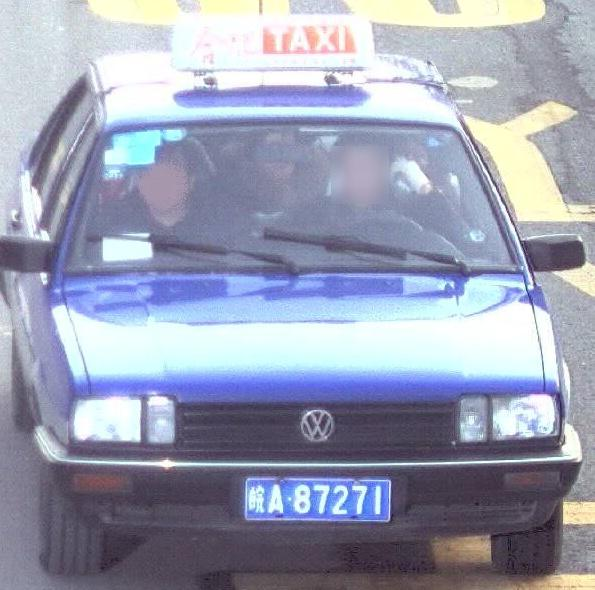
\includegraphics[width=.3\textwidth]{Horizontal1.jpg}}\hfill
	\subfloat[正常光照图片2]{
		\label{fig:nor2}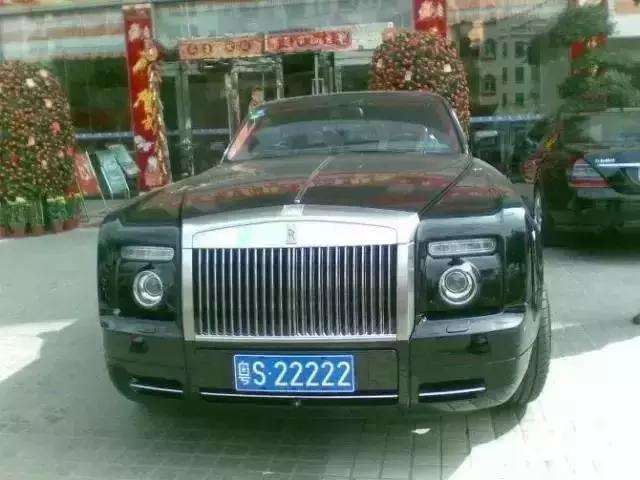
\includegraphics[width=.3\textwidth]{Horizontal2.jpg}}\hfill	
	\subfloat[正常光照图片3]{
		\label{fig:nor3}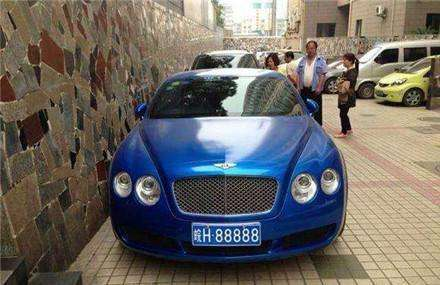
\includegraphics[width=.3\textwidth]{Horizontal3.jpg}}
	\\
	\subfloat[正常光照图片4]{
		\label{fig:nor4}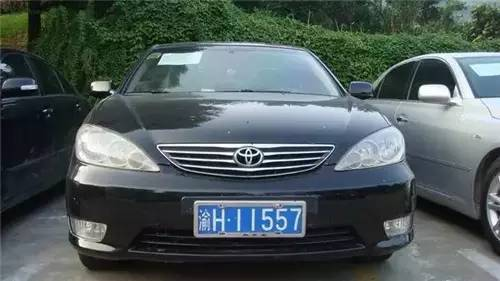
\includegraphics[width=.3\textwidth]{Horizontal4.jpg}}\hfill
	\subfloat[正常光照图片5]{
		\label{fig:nor5}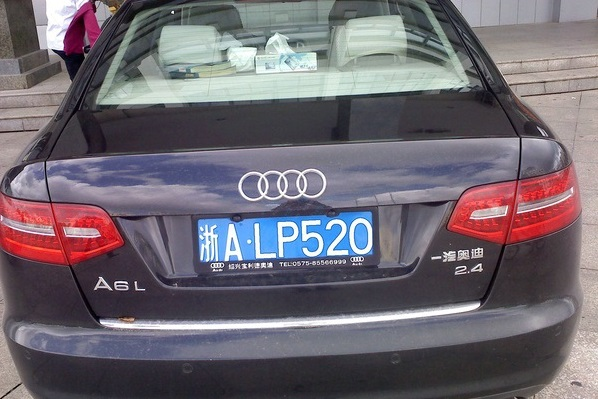
\includegraphics[width=.3\textwidth]{Horizontal5.jpg}}\hfill	
	\subfloat[正常光照图片6]{
		\label{fig:nor6}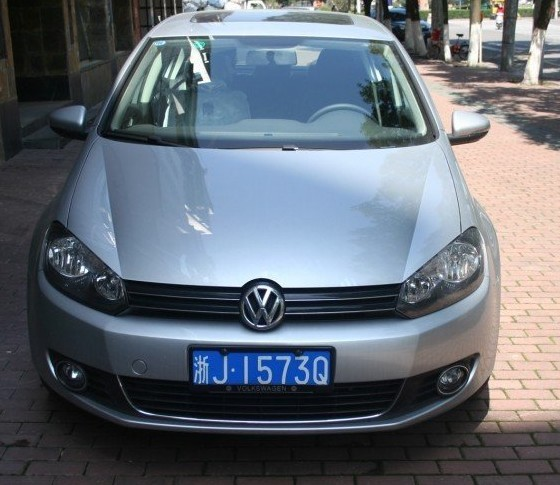
\includegraphics[width=.3\textwidth]{Horizontal6.jpg}}
	\\
	\subfloat[正常光照图片7]{
		\label{fig:nor7}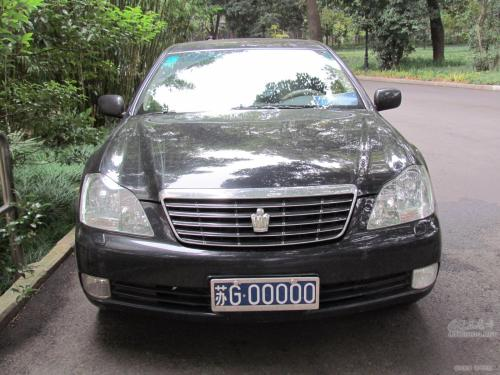
\includegraphics[width=.3\textwidth]{Horizontal7.jpg}}\hfill
	\subfloat[倾斜车牌图片1]{
		\label{fig:tilt1}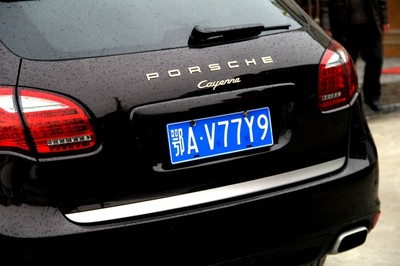
\includegraphics[width=.3\textwidth]{Inclined1.jpg}}\hfill	
	\subfloat[倾斜车牌图片2]{
		\label{fig:tilt2}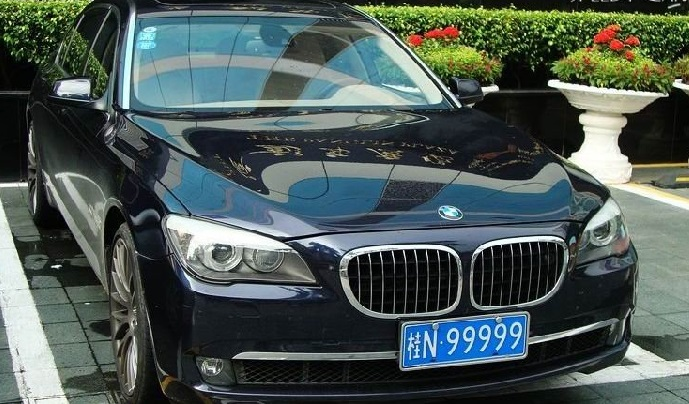
\includegraphics[width=.3\textwidth]{Inclined2.jpg}}
	\\
	\subfloat[倾斜车牌图片3]{
		\label{fig:tilt3}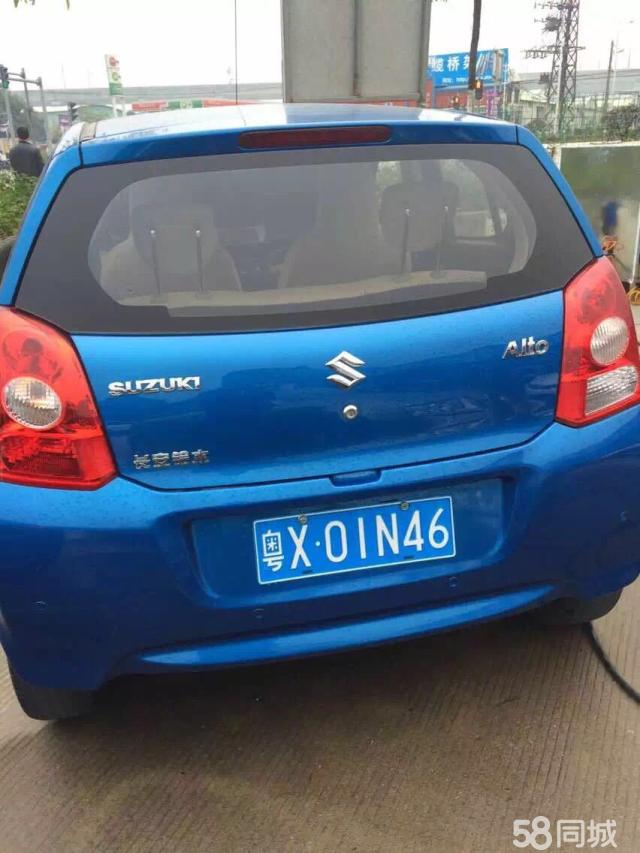
\includegraphics[width=.3\textwidth]{Inclined3.jpg}}\hfill
	\subfloat[黑暗夜景图片1]{
		\label{fig:night1}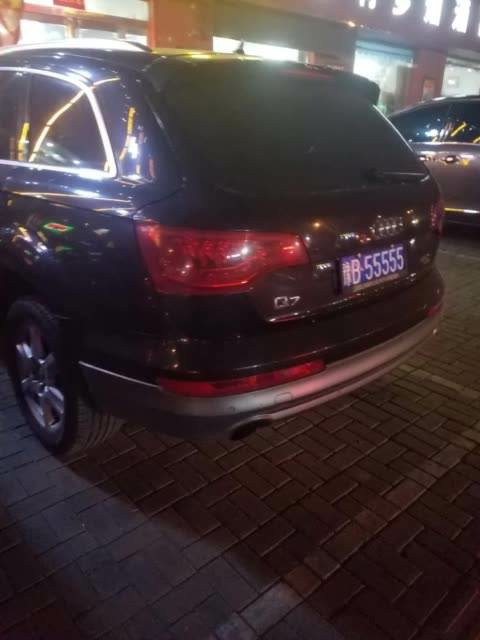
\includegraphics[width=.3\textwidth]{Night1.jpg}}\hfill	
	\subfloat[黑暗夜景图片2]{
		\label{fig:night2}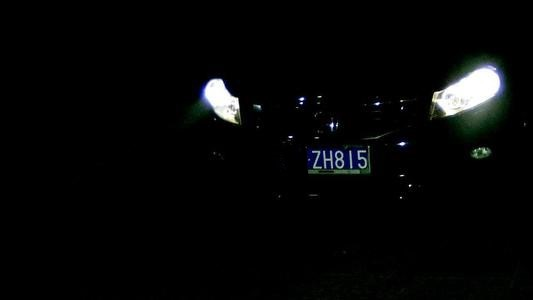
\includegraphics[width=.3\textwidth]{Night2.jpg}}
	\caption{待检测车牌图片}\label{fig:figures1}
\end{figure}

\begin{figure}[htb]
	\centering
	\subfloat[正常光照图片1结果]{
		\label{fig:nor1re}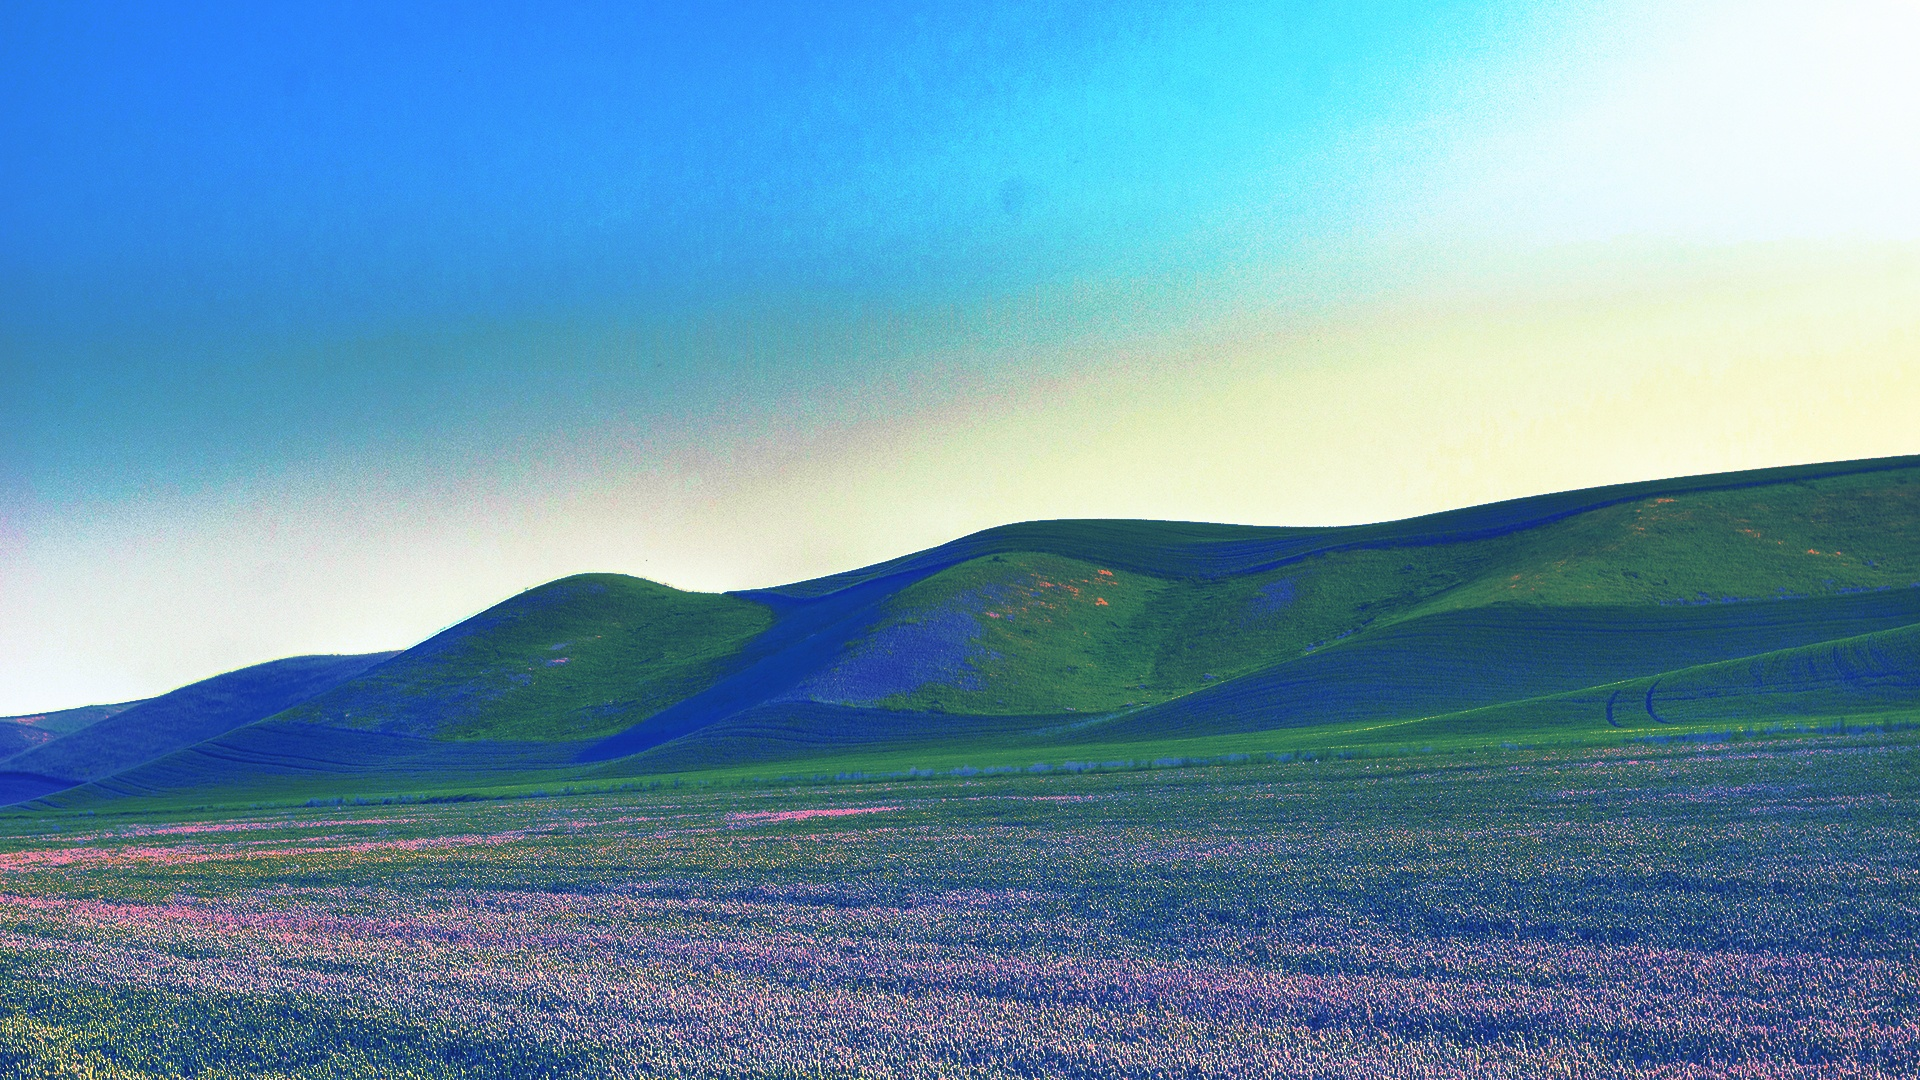
\includegraphics[width=.3\textwidth]{1.jpg}}\hfill
	\subfloat[正常光照图片2结果]{
		\label{fig:nor2re}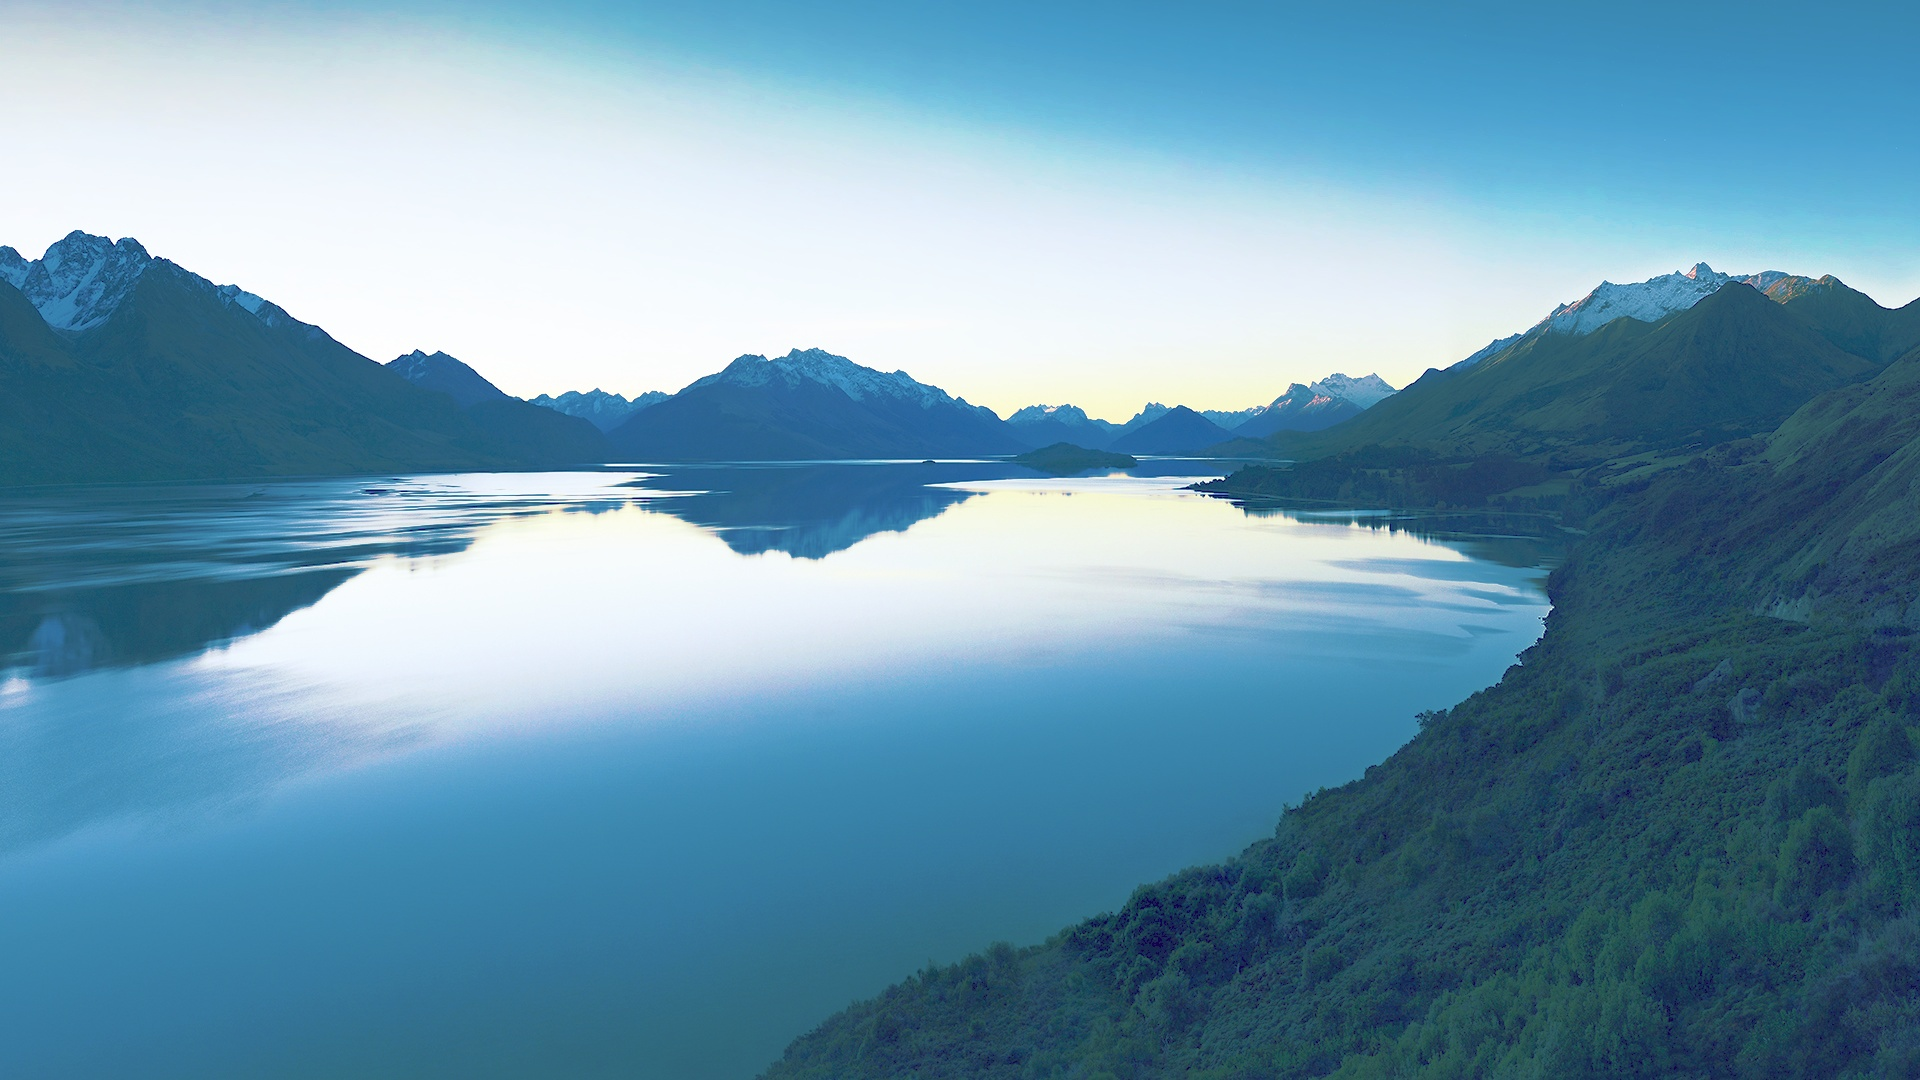
\includegraphics[width=.3\textwidth]{2.jpg}}\hfill	
	\subfloat[正常光照图片3结果]{
		\label{fig:nor3re}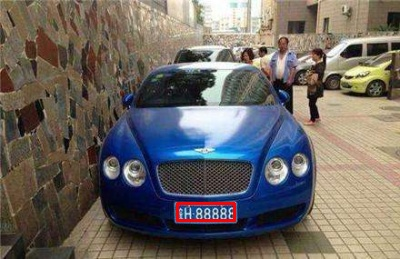
\includegraphics[width=.3\textwidth]{3.jpg}}
	\\
	\subfloat[正常光照图片4结果]{
		\label{fig:nor4re}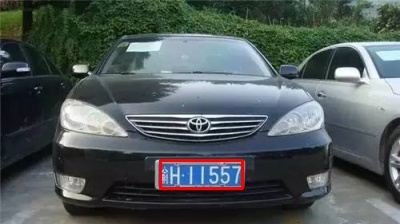
\includegraphics[width=.3\textwidth]{4.jpg}}\hfill
	\subfloat[正常光照图片5结果]{
		\label{fig:nor5re}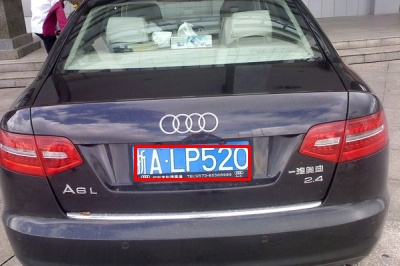
\includegraphics[width=.3\textwidth]{5.jpg}}\hfill	
	\subfloat[正常光照图片6结果]{
		\label{fig:nor6re}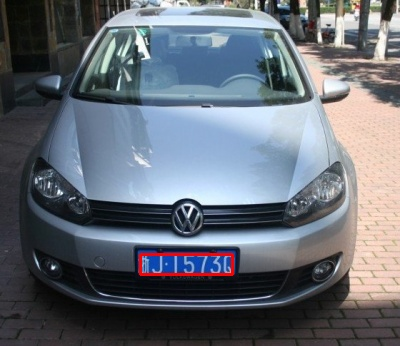
\includegraphics[width=.3\textwidth]{6.jpg}}
	\\
	\subfloat[正常光照图片7结果]{
		\label{fig:nor7re}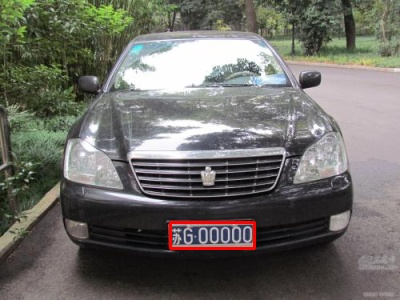
\includegraphics[width=.3\textwidth]{7.jpg}}\hfill
	\subfloat[倾斜车牌图片1结果]{
		\label{fig:tilt1re}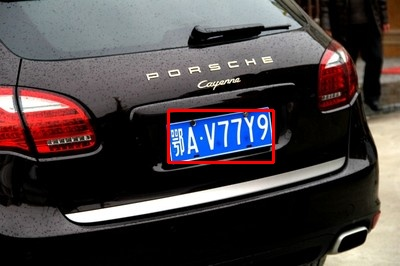
\includegraphics[width=.3\textwidth]{8.jpg}}\hfill	
	\subfloat[倾斜车牌图片2结果]{
		\label{fig:tilt2re}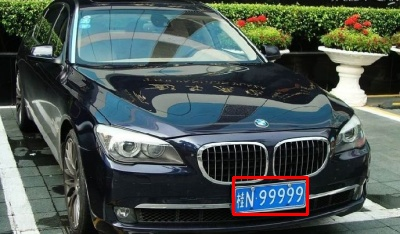
\includegraphics[width=.3\textwidth]{9.jpg}}
	\\
	\subfloat[倾斜车牌图片3结果]{
		\label{fig:tilt3re}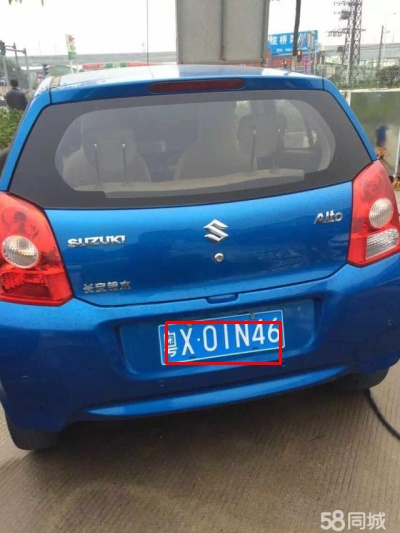
\includegraphics[width=.3\textwidth]{10.jpg}}\hfill
	\subfloat[黑暗夜景图片1结果]{
		\label{fig:night1re}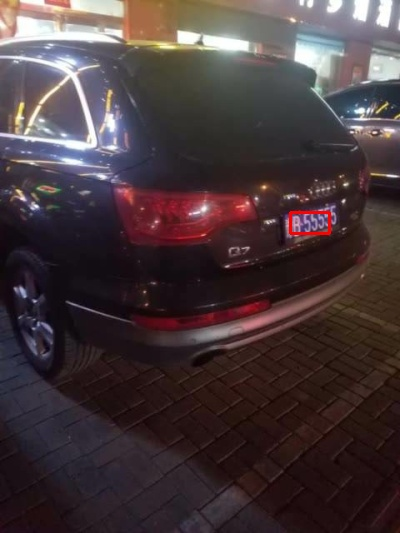
\includegraphics[width=.3\textwidth]{11.jpg}}\hfill	
	\subfloat[黑暗夜景图片2结果]{
		\label{fig:night2re}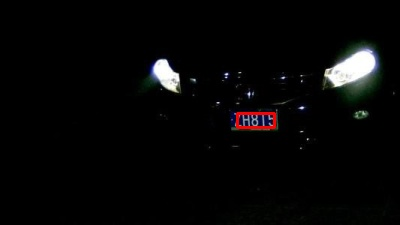
\includegraphics[width=.3\textwidth]{12.jpg}}
	\caption{车牌检测的结果}\label{fig:figures1re}
\end{figure}


\section{实验结论}

\begin{enumerate}
\item 腐蚀操作可以消除物体边界点,消除小于结构元的噪声;
\item 膨胀操作可以填补目标中的空洞,使目标增大;
\item 开运算可以平滑物体轮廓,消除平滑物体表面的“毛刺”,闭运算可以弥合狭窄的断裂,填补缝隙;
\item 顶帽变换可以补偿光照不均匀的背景亮度,从而对整幅图片进行光照均匀化处理;
\item 对于图像的形态学操作处理需要自行选用合适的参数进行处理,参数不同,得到的结果也会有很大的差异,有时甚至与预期结果相差甚远。
\end{enumerate}

\renewcommand\refname{参考文献}
 
\begin{thebibliography}{1}
\bibitem{book:li}
Rafael C. Gonzalez \& Richard E. Woods (2020). Digital Image Processing (4th ed.).

\end{thebibliography}

\newpage
\begin{appendices}

\section{检测车牌的主算法--locate\_license\_plate.py}\label{app:loc}
\begin{lstlisting}[language=python]
import numpy as np
import cv2 as cv
from src.read_file_from_dic import *


class LocatePlate(object):
    def __init__(self, img):
        self.img = img
        self.open_img = None
        self.hat_img = None

    def binaryzation(self):
        maxi = float(self.hat_img.max())
        mini = float(self.hat_img.min())
        x = maxi - ((maxi - mini) / 2)
        _, thresh = cv.threshold(self.hat_img, x, 255, cv.THRESH_BINARY)
        return thresh

    @staticmethod
    def find_rectangle(contour):
        x = []
        y = []
        for p in contour:
            y.append(p[0][0])
            x.append(p[0][1])
        return [min(x), max(x), min(y), max(y)]

    def filter_img(self):
        mask = 400 * self.img.shape[0] / self.img.shape[1]
        self.img = cv.resize(self.img, (400, int(mask)), interpolation=cv.INTER_AREA)
        gray_img = cv.cvtColor(self.img, cv.COLOR_BGR2GRAY)
        radius = 16
        height = width = radius * 2 + 1
        kernel = np.zeros((height, width), np.uint8)
        cv.circle(kernel, (radius, radius), radius, 1, -1)
        # 开运算
        open_img = cv.morphologyEx(gray_img, cv.MORPH_OPEN, kernel)
        self.open_img = open_img
        # show_img("open img", self.open_img)
        # 顶帽变换
        hat_img = cv.absdiff(gray_img, self.open_img)
        # show_img("hat img", hat_img)
        self.hat_img = hat_img
        # 二值化
        binary_img = self.binaryzation()
        # Canny边缘检测
        canny = cv.Canny(binary_img, binary_img.shape[0], binary_img.shape[1])
        # show_img("canny", canny)
        kernel = np.ones((5, 19), np.uint8)
        # 闭运算
        close_img = cv.morphologyEx(canny, cv.MORPH_CLOSE, kernel)
        # show_img("close img", close_img)

        # 开运算
        open_img = cv.morphologyEx(close_img, cv.MORPH_OPEN, kernel)
        # show_img("open img", open_img)

        # 开运算
        kernel = np.ones((14, 6), np.uint8)
        open_img = cv.morphologyEx(open_img, cv.MORPH_OPEN, kernel)
        self.open_img = open_img
        # show_img("open img", self.open_img)

    def detect_edge(self):
        contours, _ = cv.findContours(self.open_img, cv.RETR_EXTERNAL, cv.CHAIN_APPROX_SIMPLE)
        block = []
        for c in contours:
            r = self.find_rectangle(c)
            block.append(r)
        max_weight = 0
        max_index = -1
        for i in range(len(block)):
            b = self.img[block[i][0]: block[i][1], block[i][2]: block[i][3]]
            # 转化为hsv颜色空间
            hsv_img = cv.cvtColor(b, cv.COLOR_BGR2HSV)
            # 蓝色下界
            lower = np.array([100, 50, 50])
            # 蓝色上界
            upper = np.array([140, 255, 255])
            mask = cv.inRange(hsv_img, lower, upper)
            w1 = 0
            for m in mask:
                w1 += m / 255
            w2 = 0
            for n in w1:
                w2 += n
            if w2 > max_weight:
                max_index = i
                max_weight = w2
        # print(block)
        # print(max_index)
        if max_index == -1:
            return self.img
        rect = block[max_index]
        img = self.img.copy()
        cv.rectangle(img, (rect[3], rect[1]), (rect[2], rect[0]), (0, 0, 255), 2)
        # show_img("img", img)
        return img

    def locate_plate_main(self):
        self.filter_img()
        img = self.detect_edge()
        return img


def main():
    img_list = read_file_from_dic()
    for i in range(img_list.size):
        # show_img("i", img_list[i])
        print("detect img " + str(i + 1))
        locate = LocatePlate(img_list[i])
        img = locate.locate_plate_main()
        write_img_to_file(str(i + 1), img)


if __name__ == '__main__':
    main()


\end{lstlisting}

\section{从系统中读取图片并显示保存结果--read\_file\_from\_dic.py}\label{app:read}
\begin{lstlisting}[language=python]
import os
import numpy as np
import cv2 as cv


def read_file_from_dic():
    file_dir_path = '../data/'
    pic_list = []
    file_list = os.listdir(file_dir_path)
    for file in file_list:
        file_path = os.path.join(file_dir_path, file)
        print("open figure " + file_path)
        with open(file_path) as f:
            img = cv.imread(file_path)
        pic_list.append(img)
    return np.asarray(pic_list)


def show_img(title, img):
    cv.namedWindow(title, cv.WINDOW_FREERATIO)
    cv.imshow(title, img)
    cv.waitKey()
    cv.destroyAllWindows()


def write_img_to_file(file_name, img):
    file_path = '../result/' + file_name + '.jpg'
    cv.imwrite(file_path, img)

\end{lstlisting}

\end{appendices}

\end{document}
